\chapter{BACKGROUND}\label{chap:BACKGROUND}
\hspace{0.5in}This project is inspired by the research "Face Swapping: Automatically Replacing Faces in Photographs" by Dmitri Bitouk et al\cite{Bitouk2008}. In order to develop the Face Replacement System, there are several steps needed to be done.

The challenge of each step is to use practical methods to achieve the desired result. There are several approaches, developed by other researchers, which we select to use in the system. The following are the challenges we will discuss.

\section{Getting Face Contour}
\hspace{0.5in}In this project, we need to define a boundary of both the source face region and the target face region. In order to clone a face patch to fill in another head region, the two regions should be identical in shape. There are many approaches to define these regions.

One approach is to draw the face boundary manually by the user. This requires a lot of user intervention. It is a standard method that is provided in many image editing tools. It is also hard to set some constraints like the number of vertices.

Another technique is to select a region by color. This approach needs less user intervention than the previous approach. One example is being used by Adobe Photoshop as a tool named "Magic Wand Tool". The tool will start the region from the point where the user specifies, then expand to nearby pixels until the color difference from the starting point exceeds the difference threshold. It is hard to get the same shape in both the source and the target regions. Interactive Digital Photomontage \cite{Agarwala2004} uses a similar approach with graph-cut optimization.

\begin{figure}[htb]
   \centering
   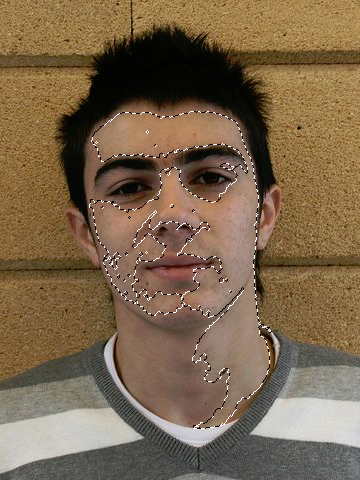
\includegraphics[width=4cm]{MagicWand.png}
   \caption{Magic Wand Tool in Adobe Photoshop}
   \label{fig:MagicWand}
\end{figure}

An automatic approach might be implemented using face detection technology if the input images are high resolution and the face detector can extract feature points. The system may simply draw lines connecting those feature points automatically.

Another approach is to create a predefined shape for the face boundary. According to the fact that the human face has only little variation, i.e. two eyes, one nose, and one mouth are located at almost the same position on anyone's face, we may extract common characteristics from many faces to define a standard face boundary. We do not need a perfect boundary which separates a face from the neck and hair. We just need a boundary to achieve smooth blending, so we can create any boundary that roughly covers eyes, nose, and mouth, but excludes neck, ears, and hair. This approach can be applicable for a low resolution image in which only the eyes can be detected by the face detector. We may need human interaction only once to draw boundaries of training faces, and then find an average shape in relation to distance and direction of eyes, then we get converged initiation boundary data. Although Face Swapping \cite{Bitouk2008} does not clearly discuss the approach to initialize the face contour, their figure, as shown in figure~\ref{fig:Contours}, shows the same contour shape for every face. So, Bitouk's approach is probably similar to the approach above.

\begin{figure}[htb]
   \centering
   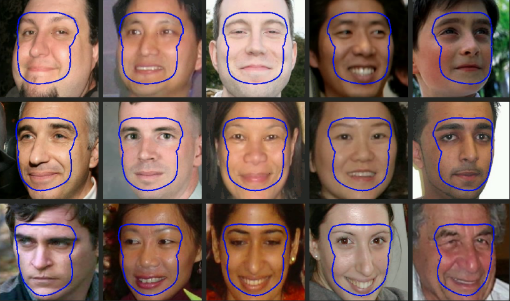
\includegraphics[width=11cm]{contours.png}
   \caption{Face Contours}
   \label{fig:Contours}
\end{figure}

When the contour is applied to the input faces, we may further modify contour to avoid crossing any prominent details.


\section{Alignment}
\hspace{0.5in}In order to do face alignment, we need to define the face position of both the source face and the target face to replace the face on the corresponding position. In the simplest way, users can manually indicate the position of eyes, nose, and mouth.

In recent past decades, artificial intelligence has been developed for many applications. One of them is face detection. "OMRON OKAO" and "OpenCV tool" are examples of face detectors that can extract feature points of a face.

\begin{figure}[htb]
   \centering
   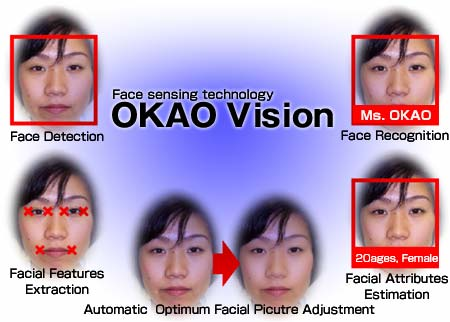
\includegraphics[width=8cm]{vision.jpg}
   \caption{Omron OKAO}
   \label{fig:Omron}
\end{figure}
\begin{figure}[htb]
   \centering
   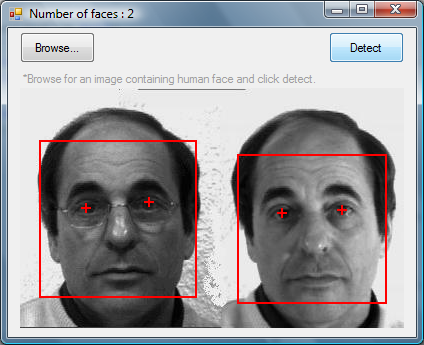
\includegraphics[width=8cm]{openCVresult.png}
   \caption{Face Detection Implementation by Zeeshan Ejaz Bhatti using OpenCV}
   \label{fig:OpenCV}
\end{figure}

After we get the feature points, we can calculate the distance between eyes, displacement between source and target face, etc.

Furthermore, some face detectors can detect the direction of pose, in pitch and yaw angles. However, it is still not accurate when detecting the direction of pose from a single image.

For the situation when the face detector is not able to detect any direction of pose, another method is to infer the pose from the position of eyes. So, the face pose can be rotated to be matched with the head pose which has been inferred. This method will also be able to infer the pose from the position of the mouth and then further adjust the face pose by skewing.

As the face patch does not lay on the appropriate position, thus, the alignment process needs to be done using the information we have discussed. There are standard methods in image processing to do transforming such as rotate, scale, skew, and translate an image in two dimensions.


\section{Relighting}
\hspace{0.5in}In order to get a more realistic result, we need two faces with similar color that can be blended smoothly. We need to do the relighting process to make the source input face have similar color and lighting as the target.

The first approach is to do a color transfer between the source input and target input images \cite{Reinhard2001}. They change the average of color and rescale the color distribution of the source image in order to have the color characteristic match the target image. However, the lighting characteristic such as level of shine cannot be transferred.

\begin{figure}[htb]
   \centering
   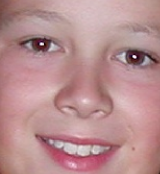
\includegraphics[width=3cm]{CTsource.png}
   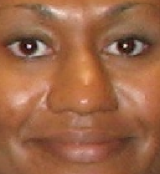
\includegraphics[width=3cm]{CTtarget.png}
   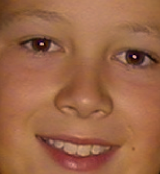
\includegraphics[width=3cm]{CToutput.png}
   \caption{Source Color, Target Color, and the Output of the Color Transfer Technique}
   \label{fig:ColorTransfer}
\end{figure}

In Face Swapping \cite{Bitouk2008}, they use nine spherical harmonics proposed by Ramamoorthi and Hanrahan which can create a realistic lighting result.

\begin{figure}[htb]
   \centering
   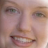
\includegraphics[width=2cm]{nonspherical.png}
   
\includegraphics[width=2cm]{spherical.png}
   \caption{The Original Lighting Condition and the Relighted Output of the Spherical Harmonics Technique}
   \label{fig:SphericalHarmonics}
\end{figure}

\section{Blending}
\hspace{0.5in}Blending is the process of mixing two images together and then making the boundary seamless. This process could finally help the result to be more realistic.

In Face Swapping \cite{Bitouk2008}, they apply feathering the face along the boundary between the images that are already similar; the well-selected images which have a similar boundary selected from a large image database.

For Poisson Image Editing \cite{Perez2003}, they use a gradient-domain technique, solving a large linear system. This method can blend any two images together and mostly get the satisfied results.

For Mean-Value Coordinates \cite{Farbman2009}, this method does not work on the gradient-domain. They improve the Poisson method efficiency by avoiding solving a large system, and also get a result that is similar to the Poisson method. 